\documentclass[titlepage]{article}

\usepackage{
    geometry,
    multicol,
    pdfpages,
    amssymb,
    graphicx
}

\geometry{
    letterpaper,
    margin=1in
}

\graphicspath{ {images/} }

\setlength{\columnsep}{0.25in}

\newenvironment{Figure}
  {\par\medskip\noindent\minipage{\linewidth}}
  {\endminipage\par\medskip}

\title{
    \textbf{
        CSCE 221 --- 200 \\
        Programming Assignment 4 \\
        Final Report
    }
}

\author{
    James Corder Guy \\
    Nathan Powell
}

\date{
    \today
}

\begin{document}
    
\includepdf[pages={-}]{./coverpage.pdf}
    \maketitle
    \begin{multicols*}{2}
        \section{Introduction}
            For this project, we implemented a fully-functional graph data structure, along with breadth-first search and Kruskal's minimum spanning tree algrorithms.
        \section{Implementation Details}
            \subsection{Graph}
                The graph was implemented using a map of vertices, a master map of edges, and an adjacency edge map for each vertex. The vertex map keys the vertices by their identifiers, and each element contains a pointer to its corresponding vertex. Each vertex is assigned a unique identifier number corresponding to the number at which it was inputted, and also a list of edges that connect to it. Both the master and the adjacency edge maps key the edges by the vertex identifier pairs that they connect, and each element contains a pointer to its corresponding edge. Each edge contains the descriptors of the two verticies it connects, and its weight. All edges are directed; in order to insert an undirected edge, two edges going in opposite directions between the same two vertices are inserted.
            \subsection{Input/Output}
                The graph pulls its initial vertices and edges from a file, reading in first the number of vertices, then the number of edges. It then reads in the next $n$ lines, where $n$ is the number of vertices, and initializes them as vertices in the vertex container. The graph then reads in the remaining lines as edges, with each line having three values, in the order of source vertex, destination vertex, and weight.
            \subsection{Breadth-First Search}
                We used a standard implementation of breadth-first search in our project. To begin, each edge and vertex in the graph is labelled as unexplored. Then, starting at the first unexplored vertex, a queue is formed, initally with the starting vertex as its only member. Then, the algorithm checks each unexplored edge connected to the starting vertex (since this is the first iteration of the algorithm, all adjacent edges are checked, since they're all unexplored). The unexplored vertices (again, all of the adjacent ones on the first iteration) are then labelled as visited, and the edges used to visit them are labelled as discovery edges. To end this iteration, each newly-visited vertex is added to the back of the queue. \par
                On the following iterations, the same procedure is repeated on the vertex currently at the front of the queue. The vertex is removed from the front, and the edges and connected vertices are checked. If an edge is found to go to an already visited vertex, it is labelled as a cross edge, and if it returns to the immediatly previous vertex (i.e., the current vertex's parent), it is labelled as a back edge. Any newly-visited vertices are then added to the queue. \par
                As each vertex is removed from the queue and processed, the algorithm updates a map, keeping track of the parent of each vertex. This allows the tree traversed by the algorithm to be constructed once the algorithm finishes running. \par
                Once all the vertices that can be reached have been processed through the queue, the queue is empty, and the algorithm checks to see if there are still any unexplored vertices in the graph, and if there are, adds the next one to the queue to begin the next iterations. These unlabelled vertices are the result of the graph either having multiple connected components, or of having a vertex that has directed nodes going only away from it. Regardless, running the algorithm again starting on each remaining unexplored vertex ensures the entire graph is labelled and added to the tree map.

			\subsection{Kruskal's Algorithm}
                         Kruskal's Algorithm was used to find the minimum spanning tree of the input graph by dividing the vertices into clusters, and then merging them back together based upon the smallest edge weights between them. These edges would make up the minimum spanning tree, and were copied into a parent map for analysis. First, The algorithm then read all the edges in the graph into a multimap, keying the edges by weight. \par
                         Next, the first and last keys in the multimap are checked; if they are the same, then every edge in the map must have the same weight; therefore, every spanning tree is a minimum spanning tree. If not, the algorithm continues and sets up containers known as clusters; these represent the vertices linked together by Krusr ekal's algorithm that will form the minimum spanning tree.\par
                         Another container that holds pointers to each cluster is initialized for constant access to each cluster. Every vertex is then inserted into its own cluster, and the algorithm begins to iterate through every edge in the multimap, comparing the vertices it connects; if they are not in the same cluster, that edge is added to the parent map, and the smaller cluster is merged into the larger cluster, though the now empty smaller cluster is not deleted; doing so would reindex the remaining clusters, invalidating all of the pointers to the clusters. This process repeats until there are $n$-1 edges in the parent map, with $n$ being the number of vertices in the graph.
		\section{Theoretical Analysis}
			\subsection{Graph}
                        Inserting an edge or vertex takes $\mathcal{O}(1)$ time, because the elements are simply added to their respective maps. Erasing an edge also takes $\mathcal{O}(1)$ time, because each edge contains the descriptors to its two vertices that can immediately access the vetices' adjacency lists. Removing a vertex takes $\mathcal{O}(m+deg(v))$ time, because every edge connected to that vertex must be deleted, as well as deleting the edge from the master edge list.
			\subsection{Input/Output}
                        The input and output both will run in $\mathcal{O}(n+m)$ time, because every vertex and every edge will have to be inserted into their respective containers, and if each individual process takes $\mathcal{O}(1)$ time, if there are n vertices and m edges then the total time will be $\mathcal{O}(n+m)$.
			\subsection{Breadth-First Search}
                        Breadth-First Search runs in $\mathcal{O}(n+m)$ time, because each vertex and edge is visited exactly twice: once to set it to UNEXPLORED, and once to set it a vertex to VISITED and an edge to either DISCOVERY or CROSS. If there are n vertices and m edges, then the total time would be $\mathcal{O}(2(n+m))$, or just $\mathcal{O}(n+m)$.
	               \subsection{Kruskal's Algorithm}
                Kruskal's Algorithm should run in $\mathcal{O}((n+m)\log{n})$ time, because each vertex will be merged at most $\log{n}$ times, resulting in $\mathcal{O}(n\log{n})$ time, because smaller clusters are always merged into larger clusters, and there will be at most $m$ removals from the edge multimap (because there are $m$ edges in total), resulting in $\mathcal{O}(m\log{n})$ time, because each union operation on the edge's vertices takes $\mathcal{O}(\log{n})$ time. Therefore, the total running time of Kruskal's Algorithm is $\mathcal{O}((n+m)\log{n})$ time.
        \section{Experimental Analysis}
            \subsection{Testing Hardware}
                Specifications of Corder's system, used for testing: \\ \\
                \begin{tabular}{r l}
                CPU:    & Intel i5-4210U @ 2.7GHz \\
                RAM:    & 8GB \\
                OS:     & Arch Linux \\
                Kernel: & 4.5.1-1 \\
                \end{tabular} \\ \\
            \subsection{Testing Procedure}
                Testing was performed with the provided timing file. There were three rounds of testing, and for each round, a different type of graph was considered: a fully-connected graph, a mesh or grid graph, and a random graph. Each round started with a small graph ($2^2$ or $2^4$, in the case of the mesh graph), and doubled in size for each consecutive test, up until the tests took a prohibitively long time to run on our hardware. Each size graph was tested 20 times, and the results were averaged. \\ \\
                Max Input Size: \\ \\
                \begin{tabular}{r l}
                Complete:   & $2^{11}$ \\
                Mesh:       & $2^{13}$ \\
                Random:     & $2^{12}$ \\
                \end{tabular}
        \section{Results}
            In each figure, the x axis is $\log_2$ (input size), and the y axis is time in ms.
            \subsection{Complete Graph}
                \begin{Figure}
                    \centering
                    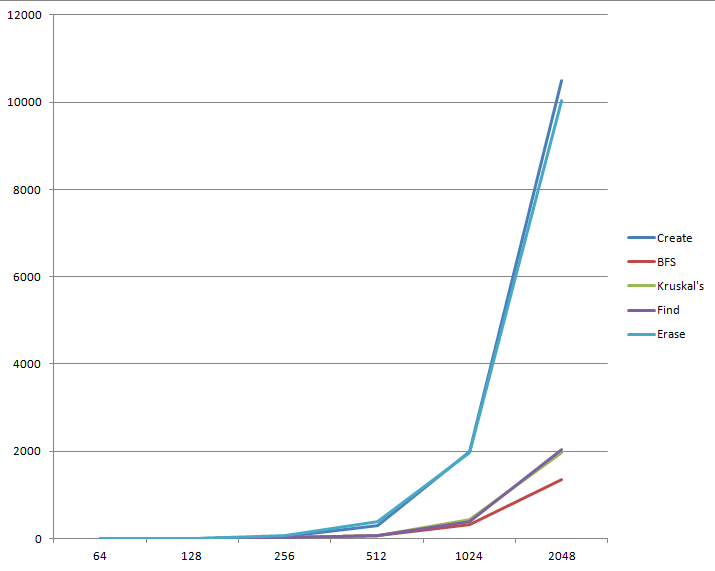
\includegraphics[width=3in]{complete}
                \end{Figure}

                \subsection{Mesh Graph}
                \begin{Figure}
                    \centering
                    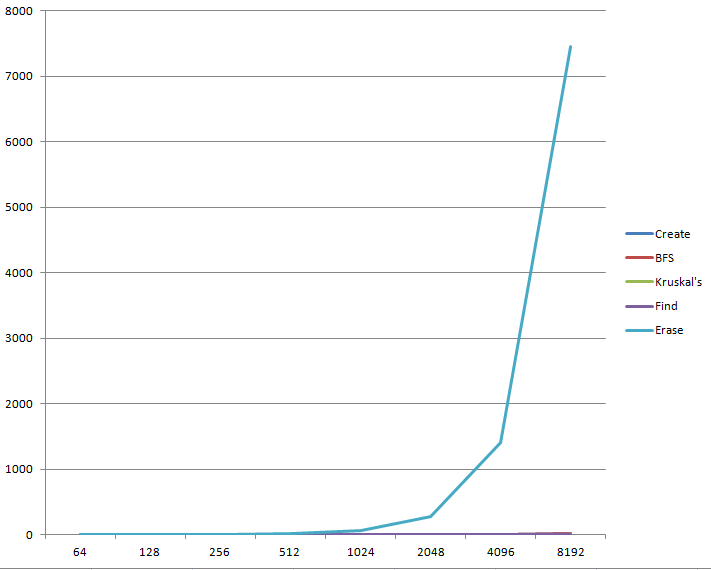
\includegraphics[width=3in]{mesh}
                \end{Figure}

                \subsection{Random Graph}
                \begin{Figure}
                    \centering
                    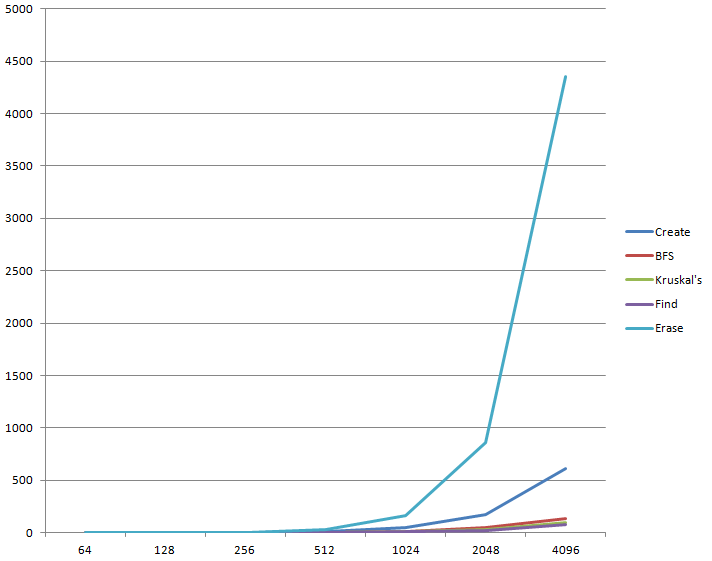
\includegraphics[width=3in]{random}
                \end{Figure}

        \section{Team Contributions}
            \subsection{Graph}
                \begin{tabular}{l l}
                    Nathan: & iterators, containers, inserters, erasers \\
                    Corder: & accessors, mutators
                \end{tabular}
            \subsubsection{Vertex}
                \begin{tabular}{l l}
                    Nathan: & adjacency list \\
                    Corder: & iterators, accessors, data members
                \end{tabular}
            \subsubsection{Edge}
                \begin{tabular}{l l}
                Corder: & iterators, accessors, data members
                \end{tabular}
            \subsubsection{I/O}
                \begin{tabular}{l l}
                   Nathan: & input \\
                   Corder: & output
                \end{tabular}
            \subsection{Algorithms}
                \begin{tabular}{l l}
                    Nathan: & Kruskal's \\
                    Corder: & BFS
                \end{tabular}
        \section{Conclusion}
            Looking at the figures, we see results consistent with our theoretical analysis. Our algorithms take much longer on the complete graph, because their time complexities are dependent on the number of edges, which is $\mathcal{O}(n^2)$ in a fully-connected graph.
    \end{multicols*}
\end{document}
